%% Scientific Conference Poster Template -- LANDSCAPE
%% tikzposter class | Landscape A0 | 3-column layout
%% Landscape orientation: for CS/ML conferences (NeurIPS, ICML, CVPR, ICLR)
%% For portrait (most other conferences), use poster.tex instead
%% Compile with: pdflatex poster-landscape.tex
%%
%% Design principles:
%%   - Landscape A0 (1189mm x 841mm), used by CS/ML conferences
%%   - 3-column layout (30/40/30), center column wider for main results
%%   - Minimal text (~500 words), maximum visual impact
%%   - tikzfigure environments (NOT standard figure) to prevent overflow
%%   - Relative sizing (linewidth-based) for all figures/charts
%%   - Generous padding (15mm+) to prevent content-edge collisions
%%   - For CVPR/NeurIPS custom sizes, add \geometry{} after \documentclass

\documentclass[25pt, a0paper, landscape, margin=15mm,
    innermargin=15mm, blockverticalspace=12mm, colspace=20mm]{tikzposter}

%% === CUSTOM PAPER SIZE (uncomment for specific conferences) ===
% \usepackage{geometry}
% % CVPR: 84"x42" (2:1 ratio)
% % \geometry{paperwidth=2133mm, paperheight=1067mm}
% % NeurIPS main: 96"x48"
% % \geometry{paperwidth=2438mm, paperheight=1219mm}
% % ICML main: 48"x36"
% % \geometry{paperwidth=1219mm, paperheight=914mm}

% Packages
\usepackage[utf8]{inputenc}
\usepackage[T1]{fontenc}
\usepackage{amsmath, amssymb}
\usepackage{graphicx}
\usepackage{booktabs}
\usepackage{enumitem}
\usepackage{pgfplots}
\pgfplotsset{compat=1.18}
\usepackage{qrcode}

% Use sans-serif for better poster readability at distance
\renewcommand{\familydefault}{\sfdefault}

% ===== COLOR SCHEME (Tech Purple + Orange accent) =====
% Modern, eye-catching, popular at ML/AI conferences
\definecolor{deeppurple}{HTML}{6D28D9}
\definecolor{lavender}{HTML}{A78BFA}
\definecolor{hotpink}{HTML}{EC4899}
\definecolor{darktext}{HTML}{1E1B4B}
\definecolor{lightbg}{HTML}{FAF5FF}

% ===== CUSTOM TITLE STYLE =====
\definetitlestyle{MLTitle}{
    width=\paperwidth, roundedcorners=0, linewidth=0pt, innersep=2cm,
    titletotopverticalspace=0mm, titletoblockverticalspace=20mm
}{
    \begin{scope}[line width=\titlelinewidth, rounded corners=\titleroundedcorners]
        \fill[color=deeppurple] (\titleposleft,\titleposbottom) rectangle (\titleposright,\titlepostop);
        % Accent gradient bar
        \fill[color=hotpink] (\titleposleft,\titleposbottom) rectangle (\titleposright,\titleposbottom+0.5cm);
    \end{scope}
}

% ===== CUSTOM BLOCK STYLE =====
\defineblockstyle{MLBlock}{
    titlewidthscale=1, bodywidthscale=1, titleleft,
    titleoffsetx=0pt, titleoffsety=0pt, bodyoffsetx=0pt, bodyoffsety=0pt,
    bodyverticalshift=0pt, roundedcorners=8, linewidth=2pt,
    titleinnersep=10mm, bodyinnersep=15mm
}{
    \draw[color=lavender!40, fill=white, rounded corners=\blockroundedcorners, line width=1pt]
        (blockbody.south west) rectangle (blockbody.north east);
    \ifBlockHasTitle
        \draw[color=deeppurple, fill=deeppurple, rounded corners=\blockroundedcorners]
            (blocktitle.south west) rectangle (blocktitle.north east);
    \fi
}

% Apply styles
\usetheme{Default}
\usetitlestyle{MLTitle}
\useblockstyle{MLBlock}

% Set colors
\colorlet{backgroundcolor}{white}
\colorlet{framecolor}{lavender}
\colorlet{titlebgcolor}{deeppurple}
\colorlet{titlefgcolor}{white}
\colorlet{blocktitlebgcolor}{deeppurple}
\colorlet{blocktitlefgcolor}{white}
\colorlet{blockbodybgcolor}{white}
\colorlet{blockbodyfgcolor}{darktext}

% Remove tikzposter watermark
\tikzposterlatexaffectionproofoff

% ===== TITLE CONTENT =====
\title{\parbox{0.90\linewidth}{\centering\textbf{%
    Scaling Transformer Attention with Sparse Mixture-of-Experts\\[0.2em]
    for Efficient Long-Context Language Modeling}}}
\author{Alice Chen$^{1}$, Bob Kumar$^{2}$, Carol Zhang$^{1}$, David Patel$^{3}$}
\institute{$^{1}$Stanford University \quad
           $^{2}$Google DeepMind \quad
           $^{3}$MIT CSAIL \\[0.3em]
           \texttt{achen@stanford.edu} \quad
           \texttt{github.com/achen/sparse-moe-attn}}

\begin{document}

\maketitle

% ===== 3-COLUMN LAYOUT (30% / 40% / 30%) =====
% Landscape poster: read left-to-right across all 3 columns
% Center column is wider for main results
\begin{columns}

    % ============================================================
    % LEFT COLUMN (30%): Background, Motivation, Method
    % ============================================================
    \column{0.30}

    \block{Motivation}{
        Standard Transformer attention scales \textbf{quadratically} ($O(n^2)$) with sequence length, limiting practical context windows to $\sim$8K tokens.

        \vspace{1em}
        \coloredbox[bgcolor=hotpink!10, fgcolor=darktext, roundedcorners=5]{%
            \textbf{Goal:} Enable 128K+ context windows with sub-quadratic compute while maintaining full attention quality.
        }

        \vspace{1em}
        \begin{itemize}[leftmargin=*, itemsep=0.6em]
            \item Long documents (books, codebases) need full context
            \item Existing sparse methods lose 2--5\% accuracy
            \item MoE approaches not yet applied to attention heads
        \end{itemize}
    }

    \block{Method: SparseMoE-Attention}{
        \vspace{0.5em}
        % Architecture diagram
        \begin{center}
        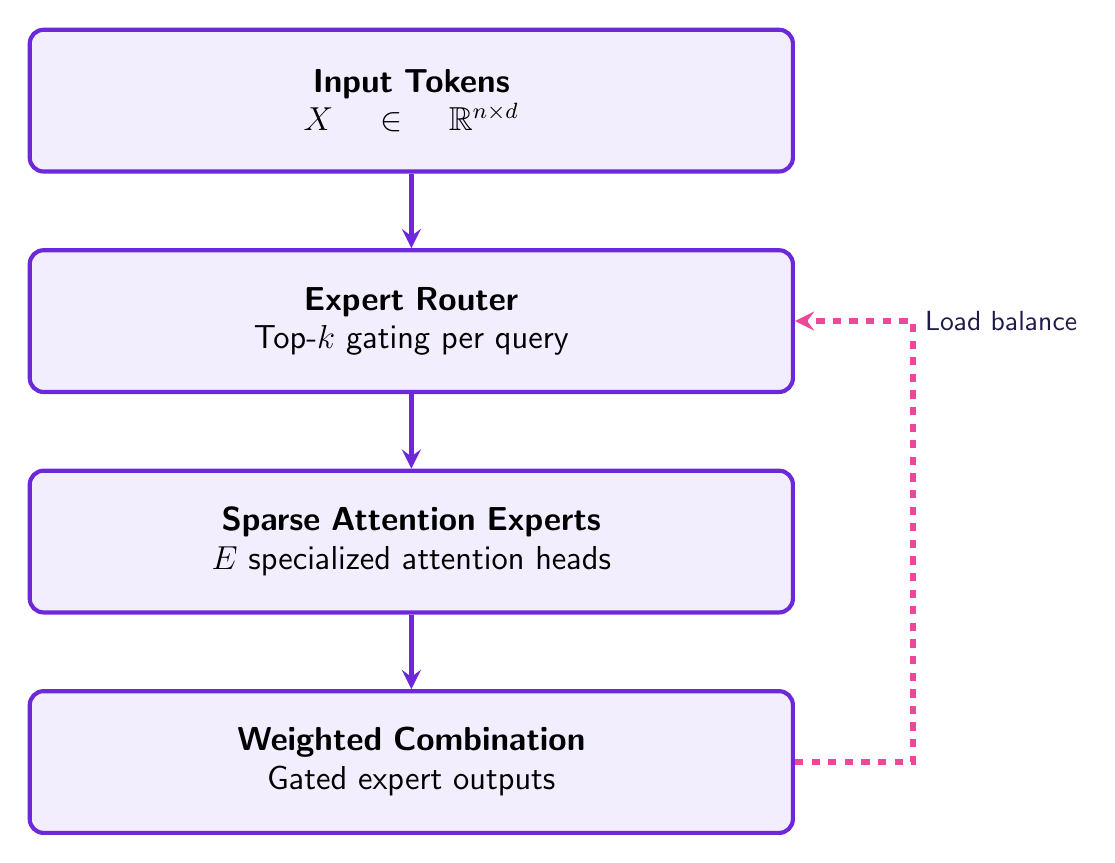
\begin{tikzpicture}[
            node distance=2.8cm,
            box/.style={rectangle, draw=deeppurple, fill=lavender!15,
                        text width=0.78\linewidth, text centered, rounded corners=5pt,
                        minimum height=1.8cm, line width=1.5pt, font=\large},
            arrow/.style={->, >=stealth, line width=2pt, color=deeppurple}
        ]
            \node[box] (input) {\textbf{Input Tokens}\\$X \in \mathbb{R}^{n \times d}$};
            \node[box, below of=input] (router) {\textbf{Expert Router}\\Top-$k$ gating per query};
            \node[box, below of=router] (experts) {\textbf{Sparse Attention Experts}\\$E$ specialized attention heads};
            \node[box, below of=experts] (combine) {\textbf{Weighted Combination}\\Gated expert outputs};

            \draw[arrow] (input) -- (router);
            \draw[arrow] (router) -- (experts);
            \draw[arrow] (experts) -- (combine);

            \draw[arrow, dashed, color=hotpink] (combine.east) -- ++(1.5cm,0) |- (router.east)
                node[midway, right, font=\normalsize, text=darktext] {Load balance};
        \end{tikzpicture}
        \end{center}

        \vspace{1em}
        \textbf{Key equation:}
        \begin{equation*}
            \text{Attn}(Q, K, V) = \sum_{i=1}^{E} g_i(Q) \cdot \text{Attn}_i(Q, K_i, V_i)
        \end{equation*}
        where $g_i$ is the expert gating weight, and each $\text{Attn}_i$ operates on a subset of keys.
    }

    \block{Training Details}{
        \vspace{0.5em}
        \begin{center}
        {\large
        \begin{tabular}{lc}
            \toprule
            \textbf{Hyperparameter} & \textbf{Value} \\
            \midrule
            Model / Experts / Top-$k$ & 7B / 16 / 4 \\
            Context / Tokens  & 128K / 1.5T \\
            Hardware        & 256$\times$ H100 \\
            \bottomrule
        \end{tabular}
        }
        \end{center}
    }


    % ============================================================
    % CENTER COLUMN (40%): Main Results (wider for emphasis)
    % ============================================================
    \column{0.40}

    \block{Main Results: Perplexity vs.\ Context Length}{
        \begin{tikzfigure}[Perplexity on PG-19 long-range benchmark across context lengths. Lower is better.]
            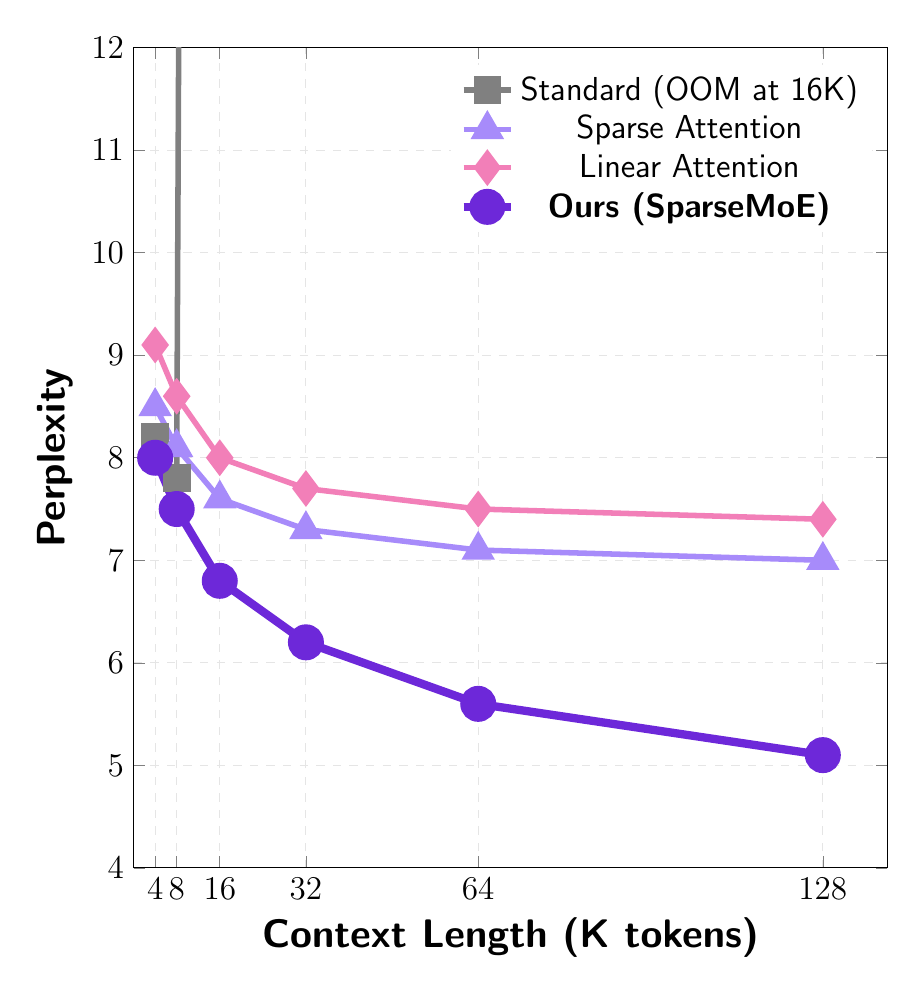
\begin{tikzpicture}
                \begin{axis}[
                    width=0.92\linewidth,
                    height=12cm,
                    xlabel={\textbf{Context Length (K tokens)}},
                    ylabel={\textbf{Perplexity}},
                    xlabel style={font=\Large},
                    ylabel style={font=\Large},
                    x tick label style={font=\large},
                    y tick label style={font=\large},
                    xmin=0, xmax=140,
                    ymin=4, ymax=12,
                    xtick={4,8,16,32,64,128},
                    grid=major,
                    grid style={dashed, gray!20},
                    legend style={at={(0.98,0.98)}, anchor=north east, font=\large, draw=none, fill=white!80}
                ]
                    % Standard Transformer
                    \addplot[color=gray, mark=square*, mark size=4pt, line width=2pt] coordinates {
                        (4, 8.2) (8, 7.8) (16, 100) (32, 100) (64, 100) (128, 100)
                    };
                    \addlegendentry{Standard (OOM at 16K)}

                    % Sparse attention baseline
                    \addplot[color=lavender, mark=triangle*, mark size=5pt, line width=2pt] coordinates {
                        (4, 8.5) (8, 8.1) (16, 7.6) (32, 7.3) (64, 7.1) (128, 7.0)
                    };
                    \addlegendentry{Sparse Attention}

                    % Linear attention
                    \addplot[color=hotpink!70, mark=diamond*, mark size=5pt, line width=2pt] coordinates {
                        (4, 9.1) (8, 8.6) (16, 8.0) (32, 7.7) (64, 7.5) (128, 7.4)
                    };
                    \addlegendentry{Linear Attention}

                    % Ours
                    \addplot[color=deeppurple, mark=*, mark size=5pt, line width=3pt] coordinates {
                        (4, 8.0) (8, 7.5) (16, 6.8) (32, 6.2) (64, 5.6) (128, 5.1)
                    };
                    \addlegendentry{\textbf{Ours (SparseMoE)}}
                \end{axis}
            \end{tikzpicture}
        \end{tikzfigure}

        \vspace{1em}
        \coloredbox[bgcolor=deeppurple!8, fgcolor=darktext, roundedcorners=5]{%
            \textbf{Key Result:} SparseMoE-Attention achieves \textbf{5.1 perplexity} at 128K context --- \textbf{27\% lower} than sparse attention and \textbf{31\% lower} than linear attention, while using only \textbf{35\% of the FLOPs} of standard attention.
        }
    }

    \block{Throughput Comparison}{
        \begin{tikzfigure}[Tokens/second at different context lengths during inference.]
            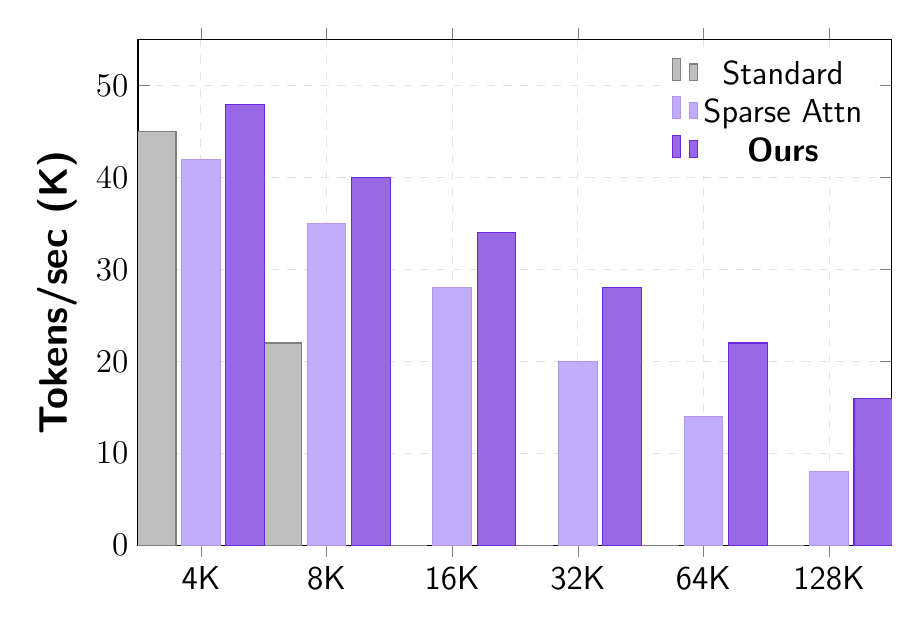
\begin{tikzpicture}
                \begin{axis}[
                    ybar,
                    bar width=14pt,
                    width=0.92\linewidth,
                    height=8cm,
                    ylabel={\textbf{Tokens/sec (K)}},
                    ylabel style={font=\Large},
                    symbolic x coords={4K, 8K, 16K, 32K, 64K, 128K},
                    xtick=data,
                    x tick label style={font=\large},
                    y tick label style={font=\large},
                    ymin=0, ymax=55,
                    legend style={at={(0.98,0.98)}, anchor=north east, font=\large, draw=none, fill=white!80},
                    enlarge x limits=0.1,
                    grid=major,
                    grid style={dashed, gray!20}
                ]
                    \addplot[fill=gray!50, draw=gray] coordinates {
                        (4K, 45) (8K, 22) (16K, 0) (32K, 0) (64K, 0) (128K, 0)
                    };
                    \addlegendentry{Standard}

                    \addplot[fill=lavender!70, draw=deeppurple!50] coordinates {
                        (4K, 42) (8K, 35) (16K, 28) (32K, 20) (64K, 14) (128K, 8)
                    };
                    \addlegendentry{Sparse Attn}

                    \addplot[fill=deeppurple!70, draw=deeppurple] coordinates {
                        (4K, 48) (8K, 40) (16K, 34) (32K, 28) (64K, 22) (128K, 16)
                    };
                    \addlegendentry{\textbf{Ours}}
                \end{axis}
            \end{tikzpicture}
        \end{tikzfigure}
    }


    % ============================================================
    % RIGHT COLUMN (30%): Analysis, Conclusions, References
    % ============================================================
    \column{0.30}

    \block{Downstream Tasks}{
        \vspace{0.5em}
        \begin{center}
        {\large
        \begin{tabular}{lccc}
            \toprule
            \textbf{Task} & \textbf{Sparse} & \textbf{Linear} & \textbf{Ours} \\
            \midrule
            SCROLLS        & 72.1  & 69.8  & \textbf{78.4}  \\
            LongBench      & 68.5  & 65.2  & \textbf{75.1}  \\
            $\infty$-Bench & 54.3  & 51.8  & \textbf{63.7}  \\
            NarrativeQA    & 71.2  & 68.9  & \textbf{76.8}  \\
            \bottomrule
        \end{tabular}
        }
        \end{center}

        \vspace{1em}
        SparseMoE-Attention outperforms all baselines by \textbf{6--9 points} on long-context benchmarks while matching standard attention on short-context tasks.
    }

    \block{Ablation: Number of Experts}{
        \begin{tikzfigure}[Effect of expert count on perplexity and FLOPs at 128K context.]
            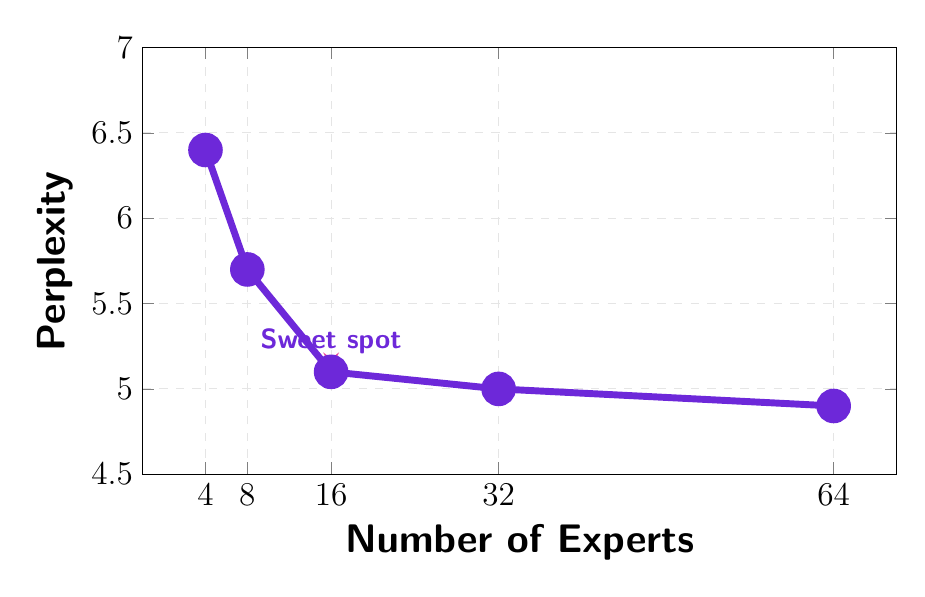
\begin{tikzpicture}
                \begin{axis}[
                    width=0.92\linewidth,
                    height=7cm,
                    xlabel={\textbf{Number of Experts}},
                    ylabel={\textbf{Perplexity}},
                    xlabel style={font=\Large},
                    ylabel style={font=\Large},
                    x tick label style={font=\large},
                    y tick label style={font=\large},
                    xtick={4,8,16,32,64},
                    ymin=4.5, ymax=7,
                    grid=major,
                    grid style={dashed, gray!20}
                ]
                    \addplot[color=deeppurple, mark=*, mark size=5pt, line width=2.5pt] coordinates {
                        (4, 6.4) (8, 5.7) (16, 5.1) (32, 5.0) (64, 4.9)
                    };

                    \node[font=\normalsize, anchor=south, color=deeppurple] at (axis cs:16, 5.15) {\textbf{Sweet spot}};
                    \draw[->, >=stealth, line width=1.5pt, color=hotpink] (axis cs:16, 5.15) -- (axis cs:16, 5.12);
                \end{axis}
            \end{tikzpicture}
        \end{tikzfigure}

        {\normalsize 16 experts: best quality/compute trade-off. Beyond 32, gains marginal ($<$0.1 PPL).}
    }

    \block{Conclusions}{
        \begin{itemize}[leftmargin=*, itemsep=0.3em]
            \item SparseMoE-Attention: \textbf{sub-quadratic} attention with \textbf{full quality}
            \item 128K context at \textbf{35\% FLOPs} of standard attention
            \item \textbf{27\% lower perplexity} than existing sparse methods
            \item Drop-in replacement for standard attention layers
        \end{itemize}
        \textbf{Future:} Multi-modal extensions, hardware-aware routing, 1M+ context.
    }

    \block{References \& Resources}{
        {\footnotesize
        [1] Vaswani+ (2017) Attention Is All You Need, \textit{NeurIPS}.
        [2] Fedus+ (2022) Switch Transformers, \textit{JMLR}.
        [3] Child+ (2019) Sparse Transformers.}
        \hfill
        \raisebox{-1cm}{\qrcode[height=3cm]{https://github.com/user/sparse-moe-attn}}
    }

\end{columns}

\end{document}
